\section{Problems of Chapter 1}

\subsection*{Problem 1.1: Int64 and Float64}

Float-point numbers (Float64) are approximations of real numbers, while Int64 is for sure an integer. The main different is that if an integer can be expressed with 64 bits, it is exactly expressed. However, if your real number is irrational (which is most often the case) you cannot store it exactly on a computer. Real numbers in computers are always approximated. They are always restricted to numerical errors, specially when we have to deal with comparisons. For instance, after some calculation you end up with two numbers $A$ and $B$. If they are for sure integers (Int64 indeed), you may check if they are equal using a simple command as \texttt{if A == B ...}, however, if they are Float64, the equality could fail due to possible numerical fluctuations at irrelevant decimal cases. So, a comparison should be done as \texttt{if abs(A-B) < abstol ...}, where \texttt{abstol} is a small number (say $10^{-8}$) that specifies your tolerance for the equality.


\subsection*{Problem 1.2: Bhaskara}

\begin{minted}[mathescape]{julia}
# define a function that receives a, b, c, and solve $ax^2 + bx + c = 0$
function bhaskara(a, b, c)
  # calculates $\Delta = b^2 - 4ac$
  delta = b^2 - 4a*c;
  # if $\Delta < 0$, convert it to Complex
  delta = (delta>0.0) ? delta : convert(Complex{Float64}, delta);
  r1 = (-b+sqrt(delta))/(2a); # first root
  r2 = (-b-sqrt(delta))/(2a); # second root
  return (r1, r2); # return roots as a tuple
end

# call the function Bhaskara with parameters a=2, b=-2, c=-12
# as indicated by the tuple above:
# root1 will receive the first root
# root2 will receive the second root
root1, root2 = bhaskara(2.0, -2.0, -12.0);
# print the results on screen
println("The first root is ", root1)
println("The second root is ", root2)

# testing the code for negative $\Delta$
root1, root2 = bhaskara(2.0, -2.0, +12.0);
println("The first root is ", root1)
println("The second root is ", root2)
\end{minted}

\subsection*{Problem 1.3: Scripts}

If you run your script from inside Julia using the \texttt{include} command, you have access to the variables after the code finishes, and you can use \texttt{PyPlot} to plot your data on a plot window. If you run from the BASH command line, you have to save into files, or print on the screen everything you'll need later on. 

\subsection*{Problem 1.5: Conditional evaluations}

\begin{minted}[mathescape,escapeinside=||]{julia}
using PyPlot # start the PyPlot package

# psi receives two parameters: x and a
# you could've set ``a'' globaly as well
psi(x,a) = (abs(x)>a) ? 1.0 : (x/a)^2; # ternary operator (short if)

# using a different letter for the limits just to remind you about the scopes
b = 10.0; 

xvec = linspace(-2b, 2b, 100); # x vector
# calculate psi for each x in xvec and save as a vector f
f = [ psi(x, b) for x=xvec ]; # comprehension

# plot the result
plot(xvec, f);  # $\text{see Fig. \ref{fig:probl1.5}}$
axis([-2b, 2b, 0.0, 1.1]);
\end{minted}

\begin{figure}[ht!]
 \centering
 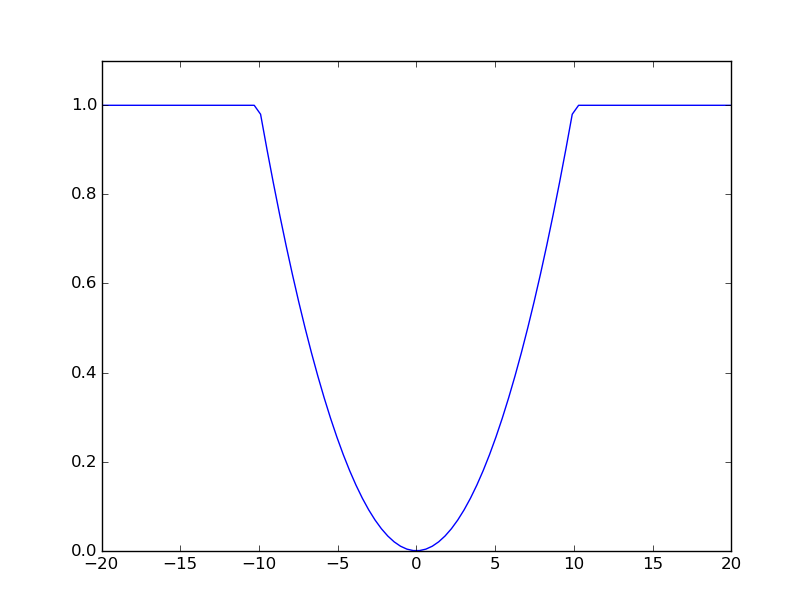
\includegraphics[width=10cm,keepaspectratio=true]{Prob-1-5.png}
 \caption{Output figure of Problem 1.5.}
 \label{fig:probl1.5}
\end{figure}

\subsection*{Problem 1.6: While and For Loops}

\begin{minted}[mathescape]{julia}
# fact receives $n$ and calculates $n!$
function fact(n::Int64)
    res = 1; # initialize the result as 1 since $n! = 1\cdot 2 \cdot 3 \cdot 4 \cdots n$
    i = n; # initialize the counter
    while i > 1 # looping from n to 1
        res = res*i; # since $n! = 1\cdot 2 \cdot 3 \cdot 4 \cdots n$
        i = i-1; # decrease counter
    end # end loop
    return res; # return the result
end

# test the code
fact(4)
\end{minted}


\subsection*{Problem 1.7: Input and Output}

\begin{minted}[mathescape]{julia}
# assuing that the content of bar.dat is
#  1.0   2.0   3.0   4.0   5.0
#  6.0   7.0   8.0   8.0   9.0
# 10.0  11.0  12.3  13.0  14.0
# 15.0  16.0  17.3  18.2  19.0
# 20.1  21.0  22.3  24.0  25.0

# a) read the CSV file
data = readcsv("bar.dat");

# and write using ; separator
writedlm("semicolon.dat", data, ';');

# b) read the ; separated file as String
data = readdlm("semicolon.dat", ';', ASCIIString);

# and write it back as text.dat
writedlm("text.dat", data);
\end{minted}


\subsection*{Problem 1.8:  Random numbers and histograms}

\begin{minted}[mathescape]{julia}
using PyPlot # start the package

list = randn(100000); # sample many random numbers
x, y = hist(list, 100); # calculate the historam with 100 bins

# x has the bin limits
# y has the bin counts
# to plot we need the bin middlepoint:
xav = (x[1:end-1] + x[2:end])/2;

# plot the histogram
plot(xav,  y);

# compare with the PyPlot :hist function
out = plt[:hist](list, 100); # also using 100 bins
x = out[2]; # equivalent to x from hist
y = out[1]; # equivalent to y from hist

# $\text{see output in Fig. \ref{fig:probl1.8}}$
\end{minted}

\begin{figure}[ht!]
 \centering
 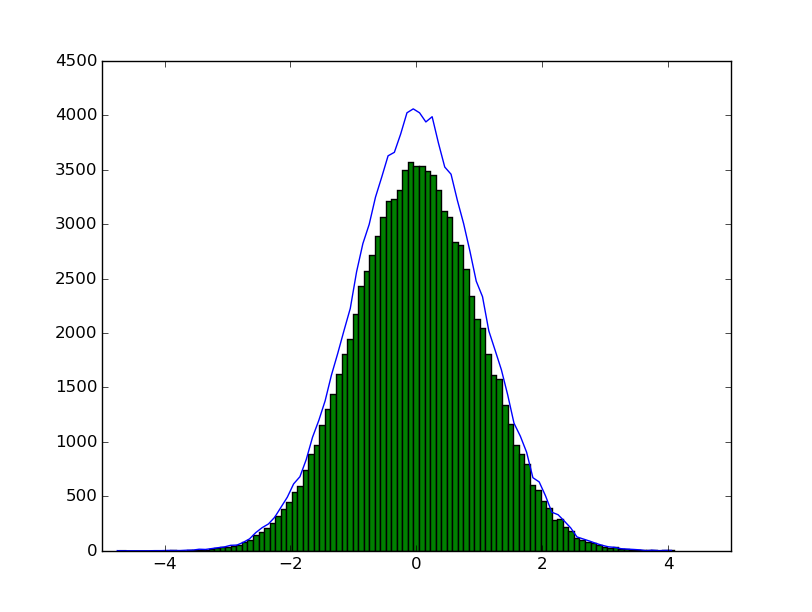
\includegraphics[width=10cm,keepaspectratio=true]{Prob-1-8.png}
 \caption{Output figure of Problem 1.8.}
 \label{fig:probl1.8}
\end{figure}


\subsection*{Problem 1.9: Cross and dot products}

\begin{minted}[mathescape]{julia}
# always use column vectors, since line vectors are seen as matrices
a = [1; 0; 0]; 
b = [0; 1; 0];
c = [5; 5; 1];

v = dot(a, cross(b,c)); # $v = a \cdot (b\times c)$
\end{minted}

\subsection*{Problem 1.10: Calculate $\pi$ using random numbers}

\begin{minted}[mathescape]{julia}
using PyPlot

# initialize vectors to store points
vecin = [0.0 0.0]; # these will be deleted afterwards
vecout = [0.0 0.0]; # these will be deleted afterwards

Pn = 0; # initilize vector to store Pi as a function of n
in=0; # initialize number of in points
out=0; # initialize number of out points
x=1:1000; # range of sampled points

for i=x # loop
    r = rand(2); # sample a point r=(x, y)
    if norm(r) <= 1 # if $|r| < 1$ the point is inside the circle
        in += 1; # increase the in counter
        vecin = [vecin; r[1] r[2]]; # store the point r=(x,y)
    else
        out += 1; # increase the out counter if point is out of the circle
        vecout = [vecout; r[1] r[2]]; # store the out point
    end
    Pn = [Pn; 4*in/(in+out)]; # recalculate pi and store each partial result
end

# the [2:end] below is used to ignore the first data from initialization

subplot(121)
plot(x, Pn[2:end]); # plot partial results as a function of n

subplot(122) # plot stored points
scatter(vecin[2:end,1], vecin[2:end,2], color="blue")
scatter(vecout[2:end,1], vecout[2:end,2], color="red") # see output in $\text{Fig. \ref{fig:probl1.10}}$

# 
\end{minted}


\begin{figure}[ht!]
 \centering
 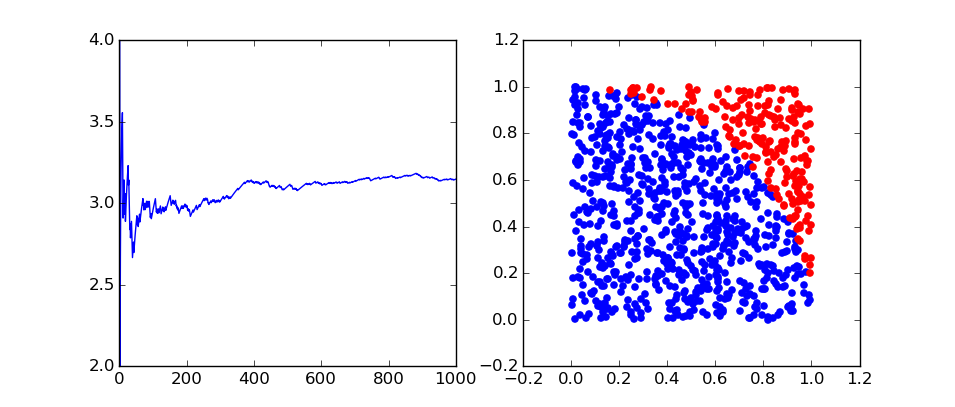
\includegraphics[width=15cm,keepaspectratio=true]{Prob-1-10.png}
 \caption{Output figure of Problem 1.10.}
 \label{fig:probl1.10}
\end{figure}



















